\documentclass{article}
\usepackage{ctex}
\usepackage{makecell}
\usepackage{graphicx}
\usepackage{geometry}
\usepackage{multirow}
\usepackage{multicol}
\usepackage{fancyhdr}
\usepackage{longtable}
\usepackage{color}
\usepackage{float}
\usepackage{listings}
\usepackage{xcolor}
\usepackage{hyperref}

\geometry{a4paper,left=25mm,right=20mm,top=25mm,bottom=25mm}

\title{程序总体框架设计报告}
\author{09021227~金桥}
\date{\today}

\lstset{
    numbers=left,
    keywordstyle= \color{ blue!70},
    commentstyle= \color{red!50!green!50!blue!50},
    rulesepcolor= \color{ red!20!green!20!blue!20} ,
    % escapeinside=``,
    numberstyle=\tt,
    numbersep=0em,
    xleftmargin=2em,
    breaklines,
    aboveskip=1em,
    framexleftmargin=2em,
    frame=shadowbox,
    basicstyle=\tt,
    language=C++
}

\begin{document}

\maketitle

\section{实验目标}

《数字图像处理》课程的后续实验包括:图像几何变换、图像灰度变换、图像增强、简易医学透视图像浏览器。
本次实验为后续实验设计总体框架(为后续实验搭建一个合理的平台,方便逐步扩展功能,避免重复编写代码),并且完成灰度图像文件的读入和显示。

·使用C++程序设计语言以及集成开发环境Qt

·\textbf{读取\texttt{bmp}格式的图像文件并完成傅里叶变换(傅里叶变换可调用现成的函数)},但所设计的程序框架要允许增加非标准格式(自定义)的图像数据文件的方法

·\textbf{框架中应允许显示多幅图像}(例如,显示处理前的图像和处理后的图像)

·总体框架着重考虑类的数据和方法的封装,以及类之间的关系

\section{程序总体框架}

程序的总体框架包括 \texttt{App}, \texttt{Core}, \texttt{ImgProvider}, \texttt{FourierTrans} 四个类。

\subsection{\texttt{App}类}

\texttt{App}类是整个程序的根本,连接后端图像处理以及前端页面展示。

\begin{lstlisting}
    class App: public QQuickView {
        Q_OBJECT
    public:
        App(QWindow *parent = 0): QQuickView(parent), _imgCore(new Core()) {...}  // 构造函数,加载 UI 界面
    public slots:
        void loadImg() {...};           // 加载图像
        void fourierTrans() {...}       // 调用 OpenCV 的傅里叶变换
        void customFourierTrans() {...} // 调用自制的傅里叶变换
        void quitApplication() {...}    // 用于退出程序的函数

    private:
        Core* _imgCore;                 // 后端处理核心
    };
\end{lstlisting}

\subsection{\texttt{Core}类}

\texttt{Core}类存储后端处理图像用到的数据。

\begin{lstlisting}
    class Core {
    public:
        Core() = default;
        // 获取图像文件的路径
        [[nodiscard]] std::string getImgPath() const {...}
        // 获取原图像内容
        [[nodiscard]] cv::Mat getOriImgMat() const {...}
        // 获取处理后图像的内容
        [[nodiscard]] cv::Mat getDstImgMat() const {...}
        // 设置处理后的图像
        void setDstImgMat(cv::Mat img) {...}
        // 从文件加载图像
        void loadImg(std::string img_path) {...}

    private:
        std::string _imgPath;  // 图像文件路径
        cv::Mat _oriImgMat;    // 原图像文件数据
        cv::Mat _dstImgMat;    // 处理后图像数据
    };
\end{lstlisting}

\subsection{\texttt{ImgProvider}类}

\texttt{ImgProvider}类用于为前端页面提供图像显示。

\begin{lstlisting}
    class ImgProvider: public QQuickImageProvider {
    public:
        ImgProvider(Core* imgCorePtr): QQuickImageProvider(QQuickImageProvider::Pixmap), _imgCore(imgCorePtr) {}
        // 为前端页面提供 QPixmap
        QPixmap requestPixmap(const QString &id, QSize *size, const QSize &requestedSize) override {...}

    private:
        // 将图像数据转换为前端显示的格式
        QPixmap cvtMat2Pixmap(const cv::Mat& mat) {...}
        Core* _imgCore;
    };
\end{lstlisting}

\subsection{\texttt{FourierTrans}类}

\texttt{FourierTrans}类用于计算傅里叶变换。自制傅里叶变换原理参见第 \ref{fft} 节。

\begin{lstlisting}
    class FourierTrans {
    public:
        // 使用 OpenCV 实现傅里叶变换,速度较快
        [[nodiscard]] cv::Mat fourierTrans(cv::Mat srcImage) {...}
        // 自制傅里叶变换,速度较慢
        [[nodiscard]] cv::Mat customFourierTrans(const cv::Mat &srcImg) {...}
    private:
        const double _pi = 3.1415926535897932;
    };
\end{lstlisting}

\section{运行示例}

以对图像进行傅里叶变换为例。

首先打开程序,点击左上角文件图标,选择\texttt{bmp}文件导入,导入之后如图所示。左侧展示的是未处理的图像,右侧是处理后的图像。

\begin{figure}[H]
    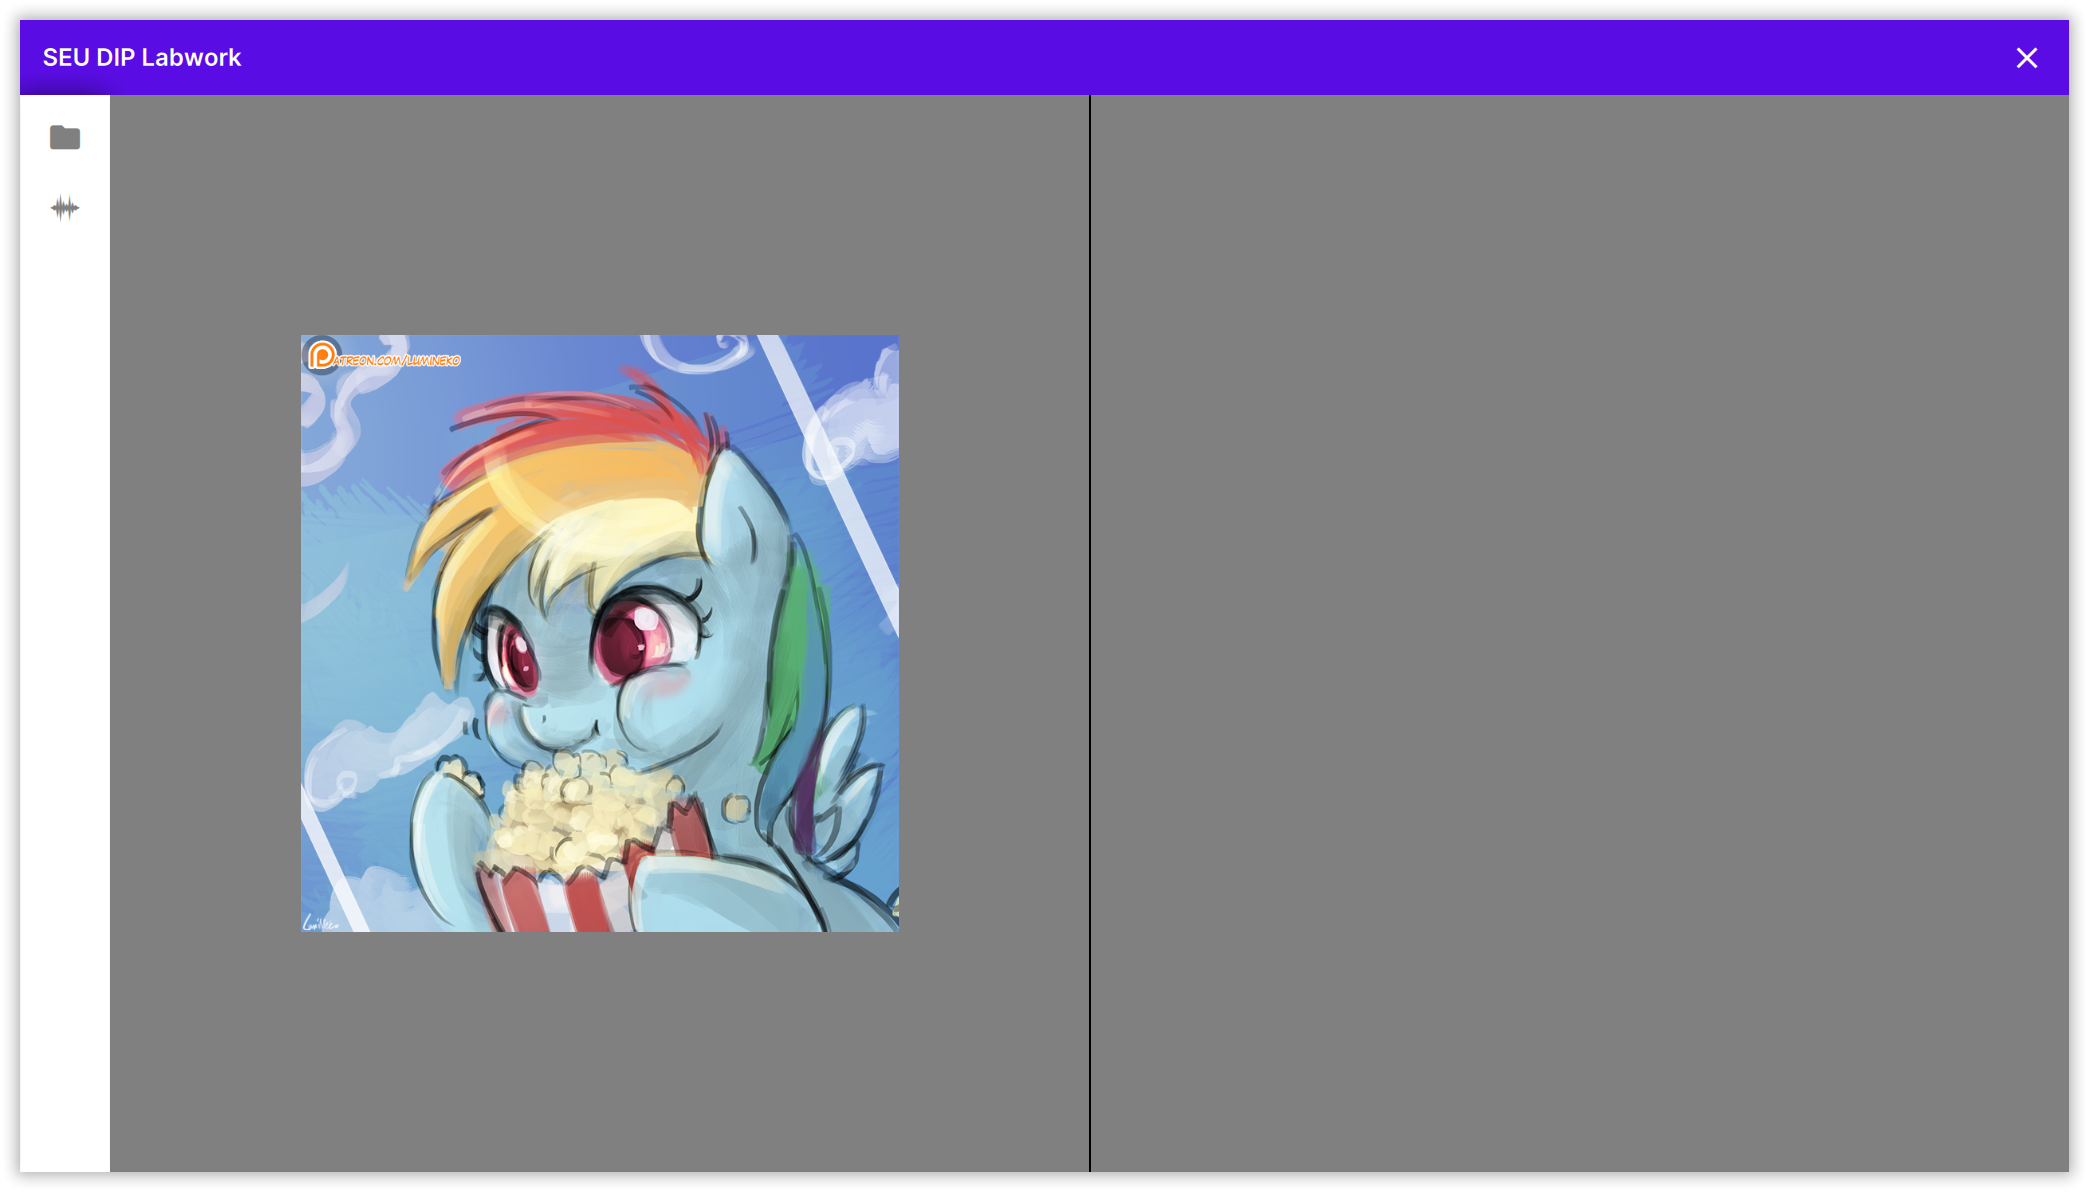
\includegraphics[width=\textwidth]{img/usage-1.png}
\end{figure}

点击左侧波形图标,右侧即可出现经过傅里叶变换的图像。

~~~~·\textbf{左键点击}为调用OpenCV的傅里叶变换

~~~~·\textbf{右键点击}为调用自制的傅里叶变换

两侧的图像均可鼠标拖动并使用滚轮缩放查看。

\begin{figure}[H]
    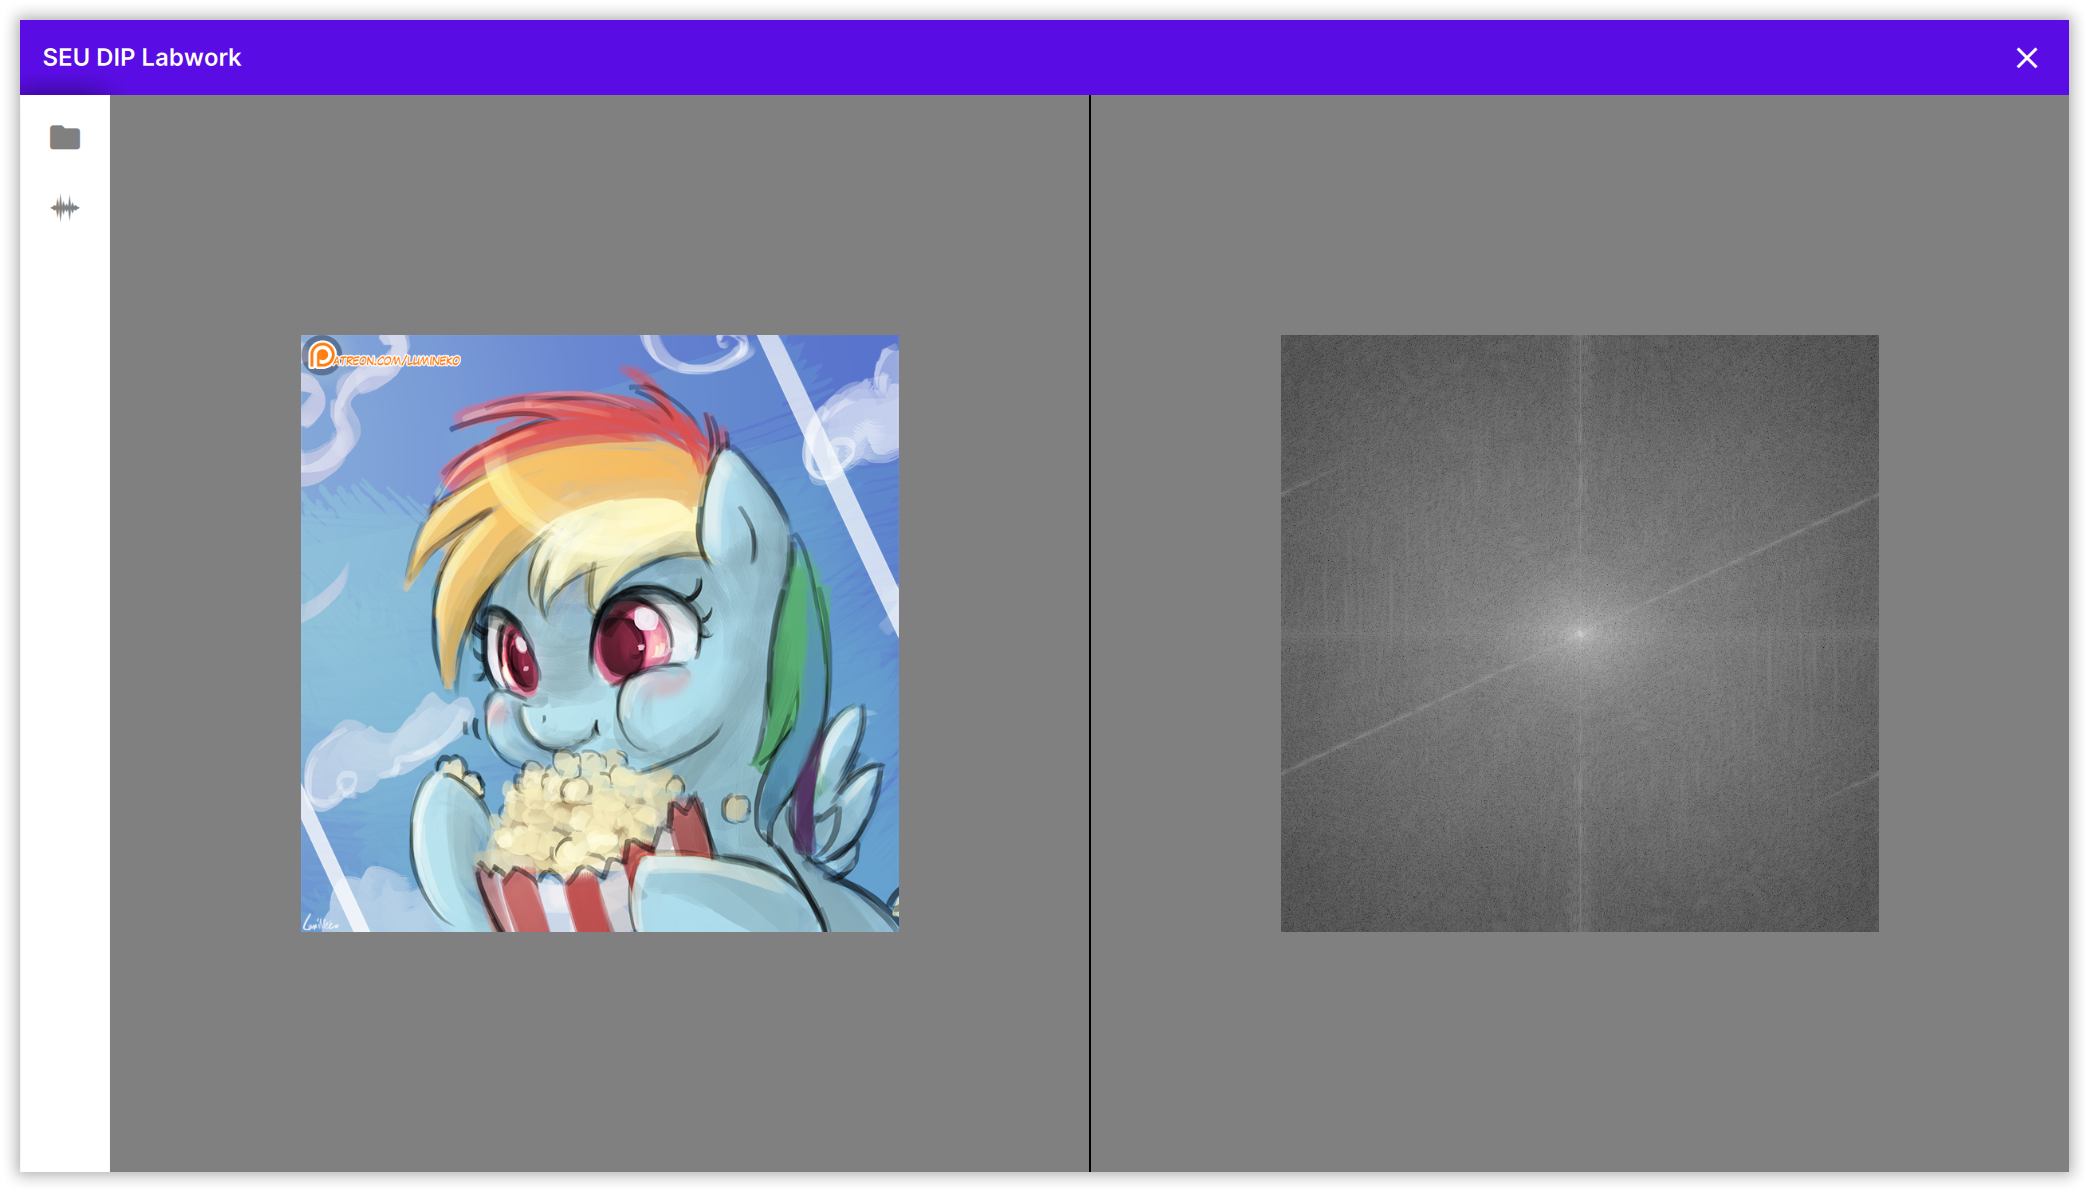
\includegraphics[width=\textwidth]{img/usage-2.png}
\end{figure}

\section{傅里叶变换}
\label{fft}

\subsection{使用OpenCV实现傅里叶变换}

通过调用 OpenCV 提供的 \texttt{dft} 函数可以方便快速的实现傅里叶变换。

\subsection{自制傅里叶变换}

通过以下二维离散傅里叶变换公式可以实现一个简易的傅里叶变换:
$$F(u, v)=\sum_{x=0}^{M-1}\sum_{y=0}^{N-1}f(x, y)e^{-j2\pi (ux/M+vy/N)}$$

首先将\texttt{cv::Mat}格式的数据转换为\texttt{double}类型的数组,之后进行两轮循环计算,每次计算再次遍历整张图像,时间复杂度为 $O(m^2n^2)$.
最后进行归一化并调整图像,使得低频位于中央即可。具体实现参照代码。

\end{document}
